\documentclass[12pt,ascmac]{jreport}
\usepackage{eclepsf}
\usepackage{tascmac}
\usepackage{url}
\usepackage{amsmath}
\usepackage[longnamesfirst]{natbib}
\usepackage{atbegshi}
\ifnum 42146=\euc"A4A2
  \AtBeginShipoutFirst{\special{pdf:tounicode EUC-UCS2}}
\else
  \AtBeginShipoutFirst{\special{pdf:tounicode 90ms-RKSJ-UCS2}}
\fi
\usepackage[dvipdfmx]{graphics}
\usepackage[dvipdfmx]{graphicx}
\usepackage[dvipdfmx]{color}
\usepackage[dvipdfmx, bookmarks=true, bookmarksnumbered=true,%
bookmarkstype=toc,%
pdftitle={Inferring parking block from vehicle position data},%
pdfsubject={},%
pdfauthor={Yasunobu Toyota},%
pdfkeywords={ITS,location information,Probe Vehicle Systems,mobile network}%
]{hyperref}

\setlength{\headheight}{-20pt} % original is 2.45mm 7pt
\setlength{\textheight}{660pt} % original is 225.75mm 645pt
\setlength{\textwidth}{441pt}
\oddsidemargin=0pt

\renewcommand{\topfraction}{.99}
\renewcommand{\textfraction}{.0}
\renewcommand{\floatpagefraction}{.99}
\renewcommand{\bibname}{参考文献}


\begin{document}

\pagenumbering{roman}

\begin{titlepage}
  \begin{center}
    \begin{large}
      卒業論文   2017年度(平成29年)\\
      \vspace{72pt}
      \textbf{自動車の位置情報ログデータを用いた\\
      駐車区画推定手法の提案}
      \end{large}
  \end{center}
  \vspace{40em}
  \begin{flushright}
    \large 慶應義塾大学 総合政策学部\\
    豊田 安信
  \end{flushright}
\end{titlepage}


卒業論文要旨 2017年度 (平成29年度)

~ \bigskip ~ \\
\begin{center}
\begin{large}
  自動車の位置情報ログデータを用いた\\
  駐車区画推定手法の提案
\end{large}
\end{center}
%## 背景$\cdot$問題提起

マイカー利用者による駐車場待ちや空き駐車場の探索により生じる交通渋滞は,日本の都市部や主要な観光地等において深刻な社会問題化している.

また,駐車場全体を目視で見渡すことの出来ない大型駐車場や階層型駐車場においても,施設への入り口や特定の店舗の近傍などの人気の高い区画に利用者が集中するため,空き状況の確認を試みる車両による渋滞が頻発する.一部の施設では超音波センサ等による常設筐体を用いて満空状況を管理する中央管理型システムが導入されているが,運営者が用意できるコストに依存している.
 
一方,近年では自律分散型制御を行うアーキテクチャも考案されている.これは利用車両に搭載された車々間通信端末によって位置情報を共有することで空き状況をセンシングするため,常設機器を必ずしも必要としない.しかし駐車場全体のネットワークモデルの事前の構築が必要になるため,結果として駐車場の運営主体による維持$\cdot$運営を必要とするという欠点がある.


そこで,本研究では駐車場内の車両の位置情報のログデータから,特定のエリアにおける駐車場全体のネットワークモデルを構築するための手法を提案する.本手法を用いることによって,駐車場内での車両の振る舞いを予測し,駐車区画の位置関係の推定が可能になる.加えて,それらのデータから学習満車時の各駐車区画の収容台数を予測することが可能となる.


この手法を評価するため,駐車区画の人気度に差があり空き区画探索の徘徊が発生しやすい慶應義塾大学湘南藤沢キャンパス内駐車場をモデルケースとし,検証実験を実施した.独自に実装した交通シミュレータ上でキャンパスを模した駐車場の仮想地図を作成し,駐車場内の各駐車区画の数や座標,駐車枠の保有台数に対して十分な推定精度を得るために必要な車両台数や時間に関する評価を通じて,本研究が提案するアルゴリズムの妥当性が証明された.

本研究が提案するネットワークモデル構築システムと既存研究で用いられた手法を活用することで,路上常設のセンサーを用いること無く,駐車場全体の空き状況の把握$\cdot$可視化$\cdot$最適な区画へのナビゲーションを行うことが可能になり,利用車両の無駄な徘徊の低減や駐車時間の減少を見込める.加えて都市部や観光地の様な同様の問題が発生しやすい環境下においても,駐車場運営主体の枠を超えた空き状況の統合的な可視化の実現と,渋滞の低減に対する取り組みがが期待される.

キーワード \\
\underline{1.ITS},
\underline{2.位置情報},
\underline{3.プローブ情報},
\underline{4. 携帯電話網}
\begin{flushright}
慶應義塾大学 総合政策学部\\
%~ \\
\begin{large}
  豊田 安信
\end{large}
\end{flushright}


\clearpage
Abstract of Bachlor's Thesis

\begin{flushright}
	Academic Year 2017
\end{flushright}

\begin{center}
	\begin{large}
		Inferring parking block from vehicle position data 
	\end{large}
\end{center}

The traffic congestion caused by searching for an empty parking lot has become a serious social problem especially in urban areas of Japan and major tourist spots.

Also, the congestion frequently occurs due to vehicles attempting to check the availability of a large parking area where you can not see the entire parking lot by visual inspection.
Some of the stores have introduced Central management type fullness management system but it is expensive so that everyone cannot afford it. 

On the other hand, an architecture that performs autonomous distributed control has been devised in recent years. This architecture does not necessarily require permanent equipment because it senses empty situation by sharing location information by Vehicle-to-Vehicle communication. However, it has the disadvantage of requiring the maintenance and operation of the parking area management entity because it is necessary to construct a network model of the entire parking area in advance.

Therefore, in this research, we propose a method for constructing the network model of the entire parking area in a specific area from the log data of the position information about vehicles in the parking area. By using this method, it is possible to predict the behavior of the vehicle in the parking lot and estimate the positional relationship of the parking section. Additionally, it is possible to predict the number of accommodated parking lots at full learning occasions from these data.

The verification experiment was carried out with Keio University Shonan Fujisawa campus parking area as a model case where there is a difference in the degree of the parking block of popularity and becomes vacant, and the loitering of the division search is easy to occur in order to evaluate this approach. We created a virtual map of a parking area imitating the campus and evaluated the generated network model on a proprietary traffic simulator. That proved the validity of the proposed algorithm.

By utilizing the proposed methods in this research, 
it becomes possible to grasp and visualize the vacancy situation of the entire parking area, and that leads to an optimized traffic volume. Even under similar environments such as urban areas and sightseeing spots where similar problems are likely to occur, there is an expectation to realize integrated visualization of vacancy situations beyond the framework of the parking management entity and efforts to reduce congestion.


Keywords :\\
\underline{1. ITS},
\underline{2. GPS},
\underline{3. Probe Vehicle Systems},
\underline{4. Mobile network},


%~ \bigskip ~ \\
\begin{flushright}
	Keio University, Faculty of Policy Management\\
	~ \\
	\begin{large}
		Yasunobu Toyota
	\end{large}
\end{flushright}


\clearpage


\tableofcontents
\clearpage

\listoffigures
\clearpage

\listoftables
\clearpage



\pagenumbering{arabic}


\chapter{序論}

\section{本研究の背景}
日本において,都市部や観光地での交通渋滞は日常的に見られる光景である.特に人気の高い施設の周辺道路では,空きのある駐車場を求める車両によって大きな渋滞を引き起こすケースがある.

\begin{figure}[htb]
	\centering
	\includegraphics[width=12cm]{fig/kokudo-fig.png}
	\caption{駐車場の空き待ち行列の発生に伴う周辺道路の渋滞の増加 \protect \footnotemark}
	\label{kokudo-fig}
\end{figure}
\footnotetext{国土交通省の配布資料より引用\cite{Kokudo}}


国土交通省の調査\cite{Kokudo}によると,一部の人気観光地において駐車場待ちによる渋滞が多発している一方で,近傍には空きのある駐車場が存在するケースが報告されている.図\ref{kokudo-fig}に駐車場の空き待ち行列の発生に伴う周辺道路の渋滞の発生をグラフに示す.

これらのような環境では,空きのある駐車場の可視化や利用者の誘導を行うシステムが求められていたが,近年では事前予約システムや空き待ち予約システムなどの試験的な導入が決まっている.その一例として,国土交通省は図\ref{kokudo-fig-2}のように周辺駐車場への誘導から交通の分散と周遊観光の拡大を目指すシステムを提案している.


\begin{figure}
	\centering
	\includegraphics[width=10cm]{fig/kokudo-fig-2.png}
	\caption{導入が進められている駐車場空き待ち予約システム \protect \footnotemark}
	\label{kokudo-fig-2}
\end{figure}
\footnotetext{国土交通省"観光地における渋滞対策"より引用\cite{Kokudo}}
しかし,これらのプラットフォームを効果的に運用するためには,各駐車場のシステムの統合的な管理$\cdot$運用が求められる.管理$\cdot$運用コストの高さから常設機器の設置が困難なため二の足を踏む駐車施設も多い.駐車場は運営者が個人$\cdot$民間$\cdot$行政とまたがるため,それぞれの駐車場に統一した設備を設置するのは大きな障壁になる.




\section{本研究の目的}
既存の駐車場満空システムでは,運営主体による積極的な投資$\cdot$運営$\cdot$管理が必要であった.すなわち,駐車場の効率化の主体はあくまで運営者にあったとも言える.


本研究では車両の位置情報と携帯電話回線網を用いて,駐車場全体のネットワークモデルを自律的に生成する手法を提案する.これにより昨今多方面で提案されていた車両のセンサーを用いる駐車場効率化手法を,運営主体の枠組みを超えて統合的に行うことが可能になる.


\section{本論文の構成}

本論文の構成を以下に示す. 
第\ref{related}章では本研究に関連する技術や先行研究を述べる.第\ref{proposal}章では本提案手法の目的と仮説,具体的なアプローチに関して述べる.第\ref{implementation}章には評価実験を行うシミュレータの実装について記述する.第\ref{evaluation}章では評価実験の概要と結果,考察について述べる.第\ref{conclusion}章では本研究のまとめを記述する.

    % 序論

\chapter{関連する技術や先行研究}
\label{related}

%関連研究では,
%* 車両のセンサーを用いる駐車場内の最適化手法
%* 車載アプリケーションプラットフォーム
%(DICOMO論文からそのままパクってくる)
%について述べる$\cdot$

ICT環境の発達によって従来の敷設センサーに頼らない駐車場の効率化が多く研究されている.
本章では駐車場の効率化手法を分類し,本提案手法が担う役割に関して記述する.

\section{駐車場空き状況センシング手法}
\label{legacy-sensing}
本節では様々な駐車場の空き状況センシング手法について記述する.
\subsection{敷設センサーによるセンシング}
日本において従来より広く導入されている手法である.運営主体によって路側に常設された機器がセンシングを行う.そのため,管理$\cdot$利活用$\cdot$情報の開示にかかるコストを運営者が負担する場合が多い.
これらのセンサーによって得られた満空情報についてどこまでの情報を開示し提供するかは運用主体の裁量で決まる.以下に主な敷設センサーを列挙する.


\begin{itemize}
					
	\item フラップ式センサー\\
	      \begin{figure}
	      	\centering
	      	\includegraphics[width=7cm]{fig/flap.png}
	      	\caption{フラップ式センサーの設置された駐車区画\protect \footnotemark}
	      	\label{flap}
	      \end{figure}
	      \footnotetext{\url{https://www.photo-ac.com/main/detail/505568}より引用 最終確認日 2018年1月17日}
	      都市部の地上型駐車場で一般に普及しているセンシング手法である(図\ref{flap}).利用車両の未払いを防ぐ働きも担っている.
	      	      	      	      	      
	\item モニタリングセンサーノード\\
	      \begin{figure}
	      	\centering
	      	\includegraphics[width=7cm]{fig/sensor-node.png}
	      	\caption{羽田空港国際線ターミナル駐車場に設定されているモニタリングセンサーノード \protect \footnotemark}
	      	\label{sensor-node}
		  \end{figure}
		  \footnotetext{羽田空港国際線ターミナル駐車場にて2017年11月撮影}
	      大型の階層型駐車場で用いられている手法である(図\ref{sensor-node}).それぞれの駐車枠上部に常設機器を設置し空き状況をセンシングする.利用者は施設内に設置されたモニターで各駐車区画の空き状況を確認出来るケースが多い.
	      	      	      	      	      
	\item 監視カメラを用いた画像認識\\
	      \begin{figure}
	      	\centering
	      	\includegraphics[width=7cm]{fig/camera.png}
	      	\caption{監視カメラによる満空情報の認識システム\protect \footnotemark}
	      	\label{camera}
	      \end{figure}
	      \footnotetext{株式会社ニチゾウテック 駐車場誘導管制設  \url{http://www.nichizotech.co.jp/products/04parking/index.html}より引用 最終確認日2017年1月17日}
	      監視カメラの映像から各区画の満空情報を認識する手法である(図\ref{camera}).近年急速に導入されている.ステレオカメラを用いる手法も研究されており,山崎ら\cite{Yamazaki}によれば従来型のシステムよりも高い精度で車両を認識することが可能になるとされている.
\end{itemize}

運営主体によっては上記のセンサーで得られた満空情報を独自のプラットフォームでユーザーに公開する場合がある.例えばタイムズ24株式会社では,自社が運営している駐車場の大まなか満空情報をWEBサービスを用いてユーザーに公開している\cite{times}.図\ref{times-fig}にタイムズ24株式会社による検索サービスのスクリーンショットを示す.一方でユーザーが同じ地域の空き駐車場を検索するためには,運営主体ごとにそれぞれ独立したWEBサイトにアクセスする必要があり利便性を欠く.また設置$\cdot$運営に関わるコストを全て運営主体が担わなくてはならないため,運営コストを割くことが出来ない学校のような非営利団体が運営する駐車場での導入は困難である.


\begin{figure}
	\centering
	\includegraphics[width=12cm]{fig/times-fig.png}
	\caption{タイムズ24株式会社 タイムズ駐車場検索 \protect \footnotemark}
	\label{times-fig}
\end{figure}
\footnotetext{\url{https://times-info.net/}より引用 最終確認日2017年1月17日}

\section{車両のセンサーを用いる駐車場内の最適化手法}
従来,駐車場内の満空管理や車両の誘導は路側に設置されたセンサーやインジケータを用いる手法が一般的であった.
しかしながら近年ではVANETや衛星測位システム,携帯電話回線網を用いる手法が提案されている.


\subsection{VANET技術}
本節ではEliasらによるサーベイ\cite{Elias}を引用し,多くの駐車場内の効率化システムを実現する技術であるVANETについての概略について述べる.




\subsubsection{概要}
車々間$\cdot$路車間で構成されるアドホックネットワークを,一般してVANET(Vehicle Adhock Network)と呼称する.
VANETに参加する車両には車載通信装置(OBU)が装備され,他のOBUや路側装置(RSU)との無線通信が可能である.
図\ref{vanet}にVANETでの通信の概要を示す.


車両のOBU同士の通信はV2V(Vehicle to Vehicle)通信と呼ばれ,タイムクリティカルな危険予知情報の伝達に用いられる.

一方で,路側に設置されたRSUとOBUとの通信はV2I(Vehicle to infrastructure)通信と呼ばれる.これは主にRTK-GPS\cite{RTK}のような数センチ単位の正確な位置情報を車両側に提供するプロトコルや,交通信号機や指示板の情報の伝達に用いられる.

また,OBU$\cdot$RSUを伝播して情報を伝える通信をルーティングベース(RB)通信と呼ぶ.RB通信を用いて駐車場内の満空状況を車両のみで伝達する手法が山下らによって提案されている\cite{Yamashita}.




\begin{figure}
	\centering
	\includegraphics[width=10cm]{fig/vanet.png}
	\caption{VANETのネットワーク図 \protect \footnotemark}
	\label{vanet}
\end{figure}
\footnotetext{Eliasらの資料\cite{Elias}より引用}


\subsubsection{想定する無線通信規格}
VANETは各国の法規制や電波環境に併せて様々な無線通信規格での運用が議論されている.

\begin{itemize}
	\item IEEE 802.11p\cite{802.11p-official}\\
	      \label{802.11p}
	      IEEEによって定められたITS用の国際的な無線通信規格である.基本的には5.9GHz帯を用いる.
	      米国を中心に標準化$\cdot$普及が行われているが,日本においてはノンストップ自動料金支払いシステム(ETC)に代表される狭域通信(DSRC)\cite{DSRC}専用として利用されるARIB STD-T75\cite{ARIB}と,周波数帯が近いため導入が遅れている\cite{802.11p-sup}.
	\item 携帯電話回線\\
	      ITUによって標準化されている2G,2.5G,3G,4Gなどの携帯電話回線網\cite{itu}は信頼性の高いセキュリティと広いカバレッジを得られるメリットがある反面,リアルタイム性に優れないというデメリットがある.一方で,近年では次世代規格である低遅延$\cdot$多数同時接続を目標とした5Gの策定も進んでおり,VANETを用いた安全運転支援や自動運転車両の遠隔制御などでの活用が期待されている\cite{5G-soumu}.
	\item Unified wireless access\\
	      ISO/TC/204/WG16\cite{iso-tc-204}にて既存の無線通信を統合的に扱うための標準仕様として策定されたのがCALM M5\cite{CALM}である.これはIEEE802.11pをベースに携帯電話回線の技術を加えて構成されており,スループットの増加や冗長化が可能になっている.
\end{itemize}



\subsection{VANETを用いた駐車場の効率化手法}
\label{sensing-by-vanet}
VANETには安全運転支援システムやプラトゥーニングなどへの応用例が目立つが,駐車場の効率化手法としても取り入れられつつある.本節ではVANETを基盤技術として用いる関連研究に関して述べる.

\subsubsection{SPARK}

R.Luらによって提案されたSPARK\cite{Spark}は,VANETを介して全ての利用車両に対して駐車場所を指定していくプラットフォームである.図\ref{spark}は本手法が用いるV2I通信を簡潔に表したものである.中央システムが利用車両に電子チケットを発行して駐車区画の占有権を与える役割の他に,その区画へのナビゲーション機能や車両盗難防止機能なども提案している.SPARKでは,電子チケットを発行した車両がそこに駐車したと仮定することで,中央システムが駐車場全体の満空情報の監視$\cdot$提供することを想定している.しかしながら,路側センサーの設置と中央システムの運営を運営主体が行う必要性があるという従来型満空センシングアーキテクチャが抱える問題をそのまま継承している.

\begin{figure}
	\centering
	\includegraphics[width=10cm]{fig/spark-1.png}
	\caption[R.Luらにより提案されたSPARK手法の概念図]{SPARK手法ではRSUを用いたV2I通信を活用することで,利用車両への駐車枠の誘導や情報提供を可能にしている \protect \footnotemark}
	\label{spark}
\end{figure}
\footnotetext{SPARKの資料\cite{Spark}より引用}


\subsubsection{V2V通信のみで情報を伝達する手法}

山下らは,車両の近接センサーによって得られた近傍駐車枠の満空情報をVANETを用いて伝達し,ネットワークに参加している車両内で駐車場全体の満空情報を共有する手法を提案している\cite{Yamashita}.各車両が路面に書かれた駐車区画番号を車載カメラによる画像認識することで位置情報を特定することを想定している.中央のシステムに頼ること無く駐車場内の効率化が図れる一方,駐車場内のネットワークモデルを前提知識として共有しているため,運営者による詳細なネットワークモデルの提供が不可欠であると言える.

\subsubsection{VANETによる位置測位と路側から情報共有によるナビゲーションシステム}

孫らは,路車間通信によって車両の位置情報から割り出された最適な駐車区画への経路を利用者にナビゲーションする手法を提案している\cite{Sun-Kenmochi}.中央のシステムがRSUを介して車両の位置情報を収集し,満空情報と駐車成功度を車両に広報する.これらの情報を基に,新しく駐車場内に進入した車両に対して,最適な駐車区画の割当$\cdot$ナビゲーションが行われる.システムを搭載した車両が少ない場合でも駐車までの時間が短縮される点が特徴である.一方,このアーキテクチャでも,事前に中央システム$\cdot$利用車両が駐車場内のネットワークモデルを把握している必要がある.



\subsection{位置情報システムと携帯電話線網を用いたセンシング手法}

近年,位置情報システムを用いたサービスやアプリケーションがより身近なものになっている.
位置情報システムで最も広く利用されているのがGPSに代表される全球測位衛星システム(GNSS)である.GPSの測位位置の誤差は通常4.9Mほどであり\cite{gps-gov},近年では準天頂衛星システム(QZSS)による補正を受けることで理論上1M以内の高精度を見込める\cite{michibiki}.また,広帯域な携帯電話回線を安価に導入できる環境が整ったことで,携帯電話回線を備えた車載機器を用いて位置情報の収集を行う手法も一般的になっている.


本項では位置情報システムと携帯電話回線網によって満空情報を推定する手法について述べる.

\subsubsection{車載センサーと携帯電話回線網を用いた路上駐車枠の空き情報検知手法}

\begin{figure}[htb]
	\centering
	\includegraphics[width=13cm]{fig/parknet.png}
	\caption{MathurらによるParknet手法の概略図 \protect \footnotemark}
	\label{parknet-fig}
\end{figure}
\footnotetext{Parknetの資料\cite{Parknet}より引用}
MathurらによるParknetプロジェクトでは,車載センサーとGPSシステムを用いて路上駐車枠をセンシングする手法を提案している\cite{Parknet}.車両から得られたそれぞれの駐車枠の満空情報を,携帯電話回線網によって中央サーバーに収集する.それらのリアルタイムな情報から,中央サーバーが都市全体の路上駐車場のネットワークモデルを構築する.


また,CoricらはParknet手法に駐車禁止枠に対する違法駐車の検知機構を取り入れたアーキテクチャを提案している\cite{Crowdsensing}.この駐車禁止検知システムでは,90パーセント程度の推定精度が確認されている.

これらの手法の優位点は,路上に設置したセンサーに頼ること無くネットワークモデルの構築を動的に行える点にある.しかし,路上駐車場のみにフォーカスされており,敷地内駐車場に関してはまだ取り組むべき余地を残している.


\subsection{位置情報ログデータを用いた道路地図の推定手法}
\label{gps-gen-map}

スマートフォンやカーナビゲーションの移動ログデータの活用方法の一つとして,移動データから地図そのものを生成$\cdot$更新する取り組みが近年注目されている.ナビゲーションサービスの提供者にとって,地図を作成する費用を軽減出来る点だけではなく,急な通行止めや道路情報の変更にリアルタイムに柔軟な対応を可能にする点も大きなメリットになる.


\subsubsection{道路地図推定手法の分類と比較}
位置情報ログデータを用いる道路地図の推定に関して,様々な手法での提案が行われているが,Biagioniらによるサーベイ\cite{Biagioni}では大別して三つのアプローチに分類している.本節ではそれらの手法の分類と特徴について述べる.


\begin{itemize}
	\item k-Means法\\
	      \begin{figure}
	      	\centering
	      	\includegraphics[width=10cm]{fig/kmeans-inf.png}
	      	\caption{k-Means法を用いる道路地図推定のフロー \protect \footnotemark}
	      	\label{k-means-inf}
          \end{figure}
          \footnotetext{Biagioniらの資料\cite{Biagioni}より引用}
	      k-Means法はForgeyらによって1965年に提唱されたクラスタリング手法である\cite{Forgy}.近年では多くの応用分野に取り入られている.道路地図の推定という文脈では,Edelkampらによって提案された手法\cite{Edelkamp}が著名である.
	      	      	      	      	      
	      図\ref{k-means-inf}に具体的なフローを示す.まず始めに,加工をしていない移動ログデータに初期シードを一定の間隔で設置し,k-Means法を用いてクラスタリングする.その後生成されたクラスターシードを,移動実績のある他のシードと結ぶことでエッジを生成する.これを繰り返すことで生成されたエッジから道路地図を推定することが出来る.
	      	      	      	      	      
	      	      	      	      	      
	\item Trace Merging法\\
	      \begin{figure}
	      	\centering
	      	\includegraphics[width=10cm]{fig/trace-merging-inf.png}
	      	\caption{Trace Merging法を用いる道路地図推定のフロー \protect \footnotemark}
	      	\label{trace-merging-inf}
          \end{figure}
          \footnotetext{Biagioniらの資料\cite{Biagioni}より引用}
	      Caoらによって提案された手法がTrace Merging法である\cite{Cao}. 
	      この手法のフローを図\ref{trace-merging-inf}に示す.始めに,収集した位置情報ログデータをそれぞれ有向グラフとして表現する.次にこのグラフから一つを任意に選択し,このグラフのエッジの近傍で方向が一致するノード数をエッジの重みとして加算していく.最終的に残ったエッジから重みの少ない物を削除する.これにより,道路地図全体のネットワーク図が得られる.
	      	      	      	      	      
	\item カーネル密度推定法\\
	      \begin{figure}
	      	\centering
	      	\includegraphics[width=10cm]{fig/kde-inf.png}
	      	\caption{カーネル密度推定を用いる道路地図推定のフロー \protect \footnotemark}
	      	\label{kde-inf}
          \end{figure}
          \footnotetext{Biagioniらの資料\cite{Biagioni}より引用}
	      Daviesらによってカーネル密度推定(以後KDE法)\cite{Ueki}を用いて道路地図推定を行う手法が提案されている\cite{Davies}.
	      	      	      	      	      
	      KDE法を用いるフローを図\ref{kde-inf}に示す.まず,元の移動ログ群からKDE法を用いて2Dヒストグラムを生成し,一定の閾値で二階長化する.生成された画像から道路の中心値群を結んで道路全体の地図を推定する.
	         	      	          
\end{itemize}

\begin{figure}[htb]
    \centering
    \includegraphics[width=10cm]{fig/inf-eval.png}
    \caption{k-Means法$\cdot$Trace Merging法$\cdot$KDE法の評価事例 \protect \footnotemark}
    \label{inf-eval}
\end{figure}
\footnotetext{{Biagioniらの資料\cite{Biagioni}より転載}}
こうした三つの手法を,実環境データにて評価した事例図\ref{inf-eval}に示す. 
                                            
ノイズの少ないログデータを用いた場合,三手法共に有効な結果を生成しているが,KDE法では移動量の少ない動線が捨象されやすいことが見て取れる.
                                        
一方,ノイズが多いログデータを用いた場合には,Trace Merging法とk-Means法では有意な類推が出来てない.他方,KDE法は捨象されている動線があるものの,真値に近い道路地図を推定していると判断可能である.
                                        
また,Biagioniらは各種法の実行時間に関しても言及している.100パターンの移動ログをデータセットとした場合,Trace Merging法が2.5時間の処理時間を要した一方で,k-Means法では73秒,KDE法では8秒と手法間で大きく差が開いている.加えて899パターンのデータセットを与えた場合において各手法の実行時間は,Trace Merging法では2.5日,k-Means法では15分,KDE法では25秒になった.締めくくりにBiagioniらはKDE法をベースとして各手法を組み合わせた新たな手法の提案について示唆している.

\subsubsection{三つの手法をあわせたアプローチについて}
Biaginiらは上記の三つの手法を組み合わせた新しいアプローチについての発表を行っている\cite{google-mouyatteta}.これによるとKDE法をベースとしたハイブリッドアプローチを用いることによって,より真値に近い道路地図の推定が可能になるとされている.


\section{車載アプリケーションプラットフォーム}
\label{ivi}
従来,自動車の情報端末はカーナビゲーションシステムとカーオーディオがその役割を担っていた.近年ではニーズの多様化やICT環境の発展によって,多くの情報からユーザーをサポートする役割も併せて求められるようになり,より高次元化されたIVI(車両情報端末) と総称される端末が登場している\cite{DICOMO}.多くのIVIプラットフォームでは,位置情報$\cdot$インターネットへのアクセス機構を備えており,自動車の情報を扱うための標準仕様の策定が活発である\cite{Ashimura}.例えば,WEB標準化団体であるW3CからはVehicle API\footnote{\url{https://www.w3.org/TR/vehicle-information-api/}}が提案されているほか,自動車メーカー各社からはスマートフォンとの連携機能を標準化するSmartDevicelink\footnote{\url{https://smartdevicelink.com/}}が提案されている.

         % 関連する技術や先行研究
\chapter{提案手法}
\label{proposal}
\section{本提案手法の位置付け}
\label{issue-to-solve}
本章では,\ref{sensing-by-vanet}項にて述べた駐車区画の満空情報を共有する手法群や利用車両のナビゲーションを行う手法群を運用する際に,前提条件となる駐車区画の位置関係や収容台数を表すネットワークモデルの自律的な推定手法について述べる.

本研究では,車両の位置情報や駐車情報の収集に際しては\ref{ivi}節で述べたような車載アプリケーションプラットフォームによって行うと想定する.これによりVANETのような専用機器を用いる手法と比較して普及の容易度を高めることが出来る.

\ref{gps-gen-map}項で述べたように,KDE法を中心とした様々なアルゴリズムを用いることで,位置情報ログデータから道路地図は安定して生成出来ることが明らかにされている.しかしながら,駐車場のネットワークモデルを構築するためには駐車区画の位置情報,駐車枠数のパラメーターが必要になる.本研究ではこれらのパラメーターの推定手法に関して検討する.


\section{用語}
本論文内で用いる用語について,以下に定義する.
また,図\ref{networkmodel-example}に本論文で定義する用語とネットワークモデルの概念図を示す.
\begin{figure}
	\centering
	\includegraphics[width=10cm]{fig/networkmodel.png}
	\caption{本研究で定義するネットワークモデルの例}
	\label{networkmodel-example}
\end{figure}
\begin{itemize}
	\item 駐車区画:車両が駐車可能な枠が隣接する場所を指す.一つの駐車区画は駐車枠を単数あるいは複数持つ.
	% parking block
	\item 駐車場:駐車区画群を持つ施設全体を示す.
	% paking area
	\item 駐車枠:車両一台を駐車出来る箇所を指す.本論文,提案手法では車両の大きさによる駐車枠の違いは考慮しない.
	% pakrking lot
	\item ネットワークモデル:座標$\cdot$駐車枠の数をパラメーターに含む駐車場内の駐車区画を表すノードと,それらを結ぶ道路を表す重み付きエッジを含むデータ構造と定義する.ネットワークグラフの形で視覚的に表現することが出来る.
	\item 交差点:複数の道路が接続されている地点を差す.駐車場をネットワークモデルとして表した場合,駐車枠を持たないノードが交差点にあたる.
\end{itemize}


\section{目的と仮説}
\label{purpose-proposal}
\subsection{本提案手法の目的}
本提案手法では既存の駐車場内効率化手法$\cdot$ネットワークモデル構築手法の諸問題に以下のように取り組む.

\subsubsection{運営主体に依存しないアーキテクチャ}
\ref{issue-to-solve}節でも述べたように,駐車場内に常設されたセンサーにより満空情報を管理する従来のアーキテクチャでは,運営主体が負担できるコストに実施性を依存していた.そのため余分な運用コストを費やすことの出来ない駐車場施設では,利用者の利便性の向上が困難であった.

また,\ref{sensing-by-vanet}項で指摘したように,車両側のセンサーを活用する手法では,ネットワークモデルの事前構築が必要という点で,結果的に運営主体による維持$\cdot$管理が必要であった.

本提案手法では,運営主体に依らない駐車場効率化手法を実現可能にするためのネットワークモデルの自律的な推定を目指す.
\subsubsection{駐車場を含めたネットワークモデルの構築}
\ref{gps-gen-map}節で述べた道路地図推定手法では,駐車場の推定には焦点が当てられていなかった.
本研究では駐車場の位置推定を可能にするアーキテクチャを提案する.

\subsubsection{敷設センサーやRSUが不要}
第\ref{related}章でも述べたように,既存の多くの駐車場最適化手法では路上側にセンサーや通信機器(RSU)を設置する必要があった.利用車両の位置情報測位システムと携帯電話回線網を用いる本提案手法では,路側に常設する機器が必ずしも必要にならない.そのため,駐車場の運営者による投資が難しい非営利施設の駐車場でも,駐車場効率化サービスを運用することが可能になる. 

%以下はまとめにFutureworkに引っ越しする予定
%\subsubsection{複数の駐車場の統合的な管理の実現}
%本論文では単一駐車場内のネットワークモデルを推定することに焦点を当てているが,本提案手法を応用することによって,複数の駐車場を含めたネットワークモデル推定へと対象の範囲を拡げる事も可能になる.
%以下はまとめにFutureworkに引っ越しする予定
%\subsubsection{変更追従性}
%\ref{sensing-by-vanet}節で述べた既存の手法群では通行止めや駐車区画配置の変更によって新たにネットワークモデルを再設定する必要があった.本手法では利用車両の実際の使用ログを収集するため,ネッ%トワークモデルの変更にある程度の追従性を持たせる設計を行うことが可能になる.


\subsection{本研究の仮説}
本研究では,\ref{issue-to-solve}節で述べたような既存の駐車場効率化手法の諸問題の解決に取り組む.
自動車の位置情報を収集$\cdot$解析することで,駐車区画の設定や最大収容台数を駐車場ごとに設定したり路側にセンサーを常設することなく、駐車区画の空き状況を収集$\cdot$可視化することが出来るようになると予想している.

\section{本提案手法の仮定と設計}
\subsection{位置情報の収集と提供}
本提案手法には駐車場を利用する車両の位置情報を収集する機構が必要になる.ここでは位置情報収集システムに関して述べる.

\subsubsection{車載器とサービスクライアント}
\ref{ivi}節で述べたような自動車用アプリケーションプラットフォーム上で動作するサービスクライアントを利用者の車両で動作させる.サービスクライアントは携帯電話回線網を用いて,自動車の位置情報をサービスサーバーに定期的に送信する.また,車両が駐車した場合にエンジンの停止を検知して駐車シグナルを同時に送信するものとする.

\subsubsection{サービスサーバー}
本提案手法では,情報を収集しネットワークモデルを推定するサービスサーバーの実装を想定する.サービスクライアントとサービスサーバ間はインターネットを介して接続される.

\subsubsection{ネットワークモデルを利用するアプリケーション}
満空情報の可視化や駐車場内のナビゲーションを行う様々なアプリケーションを運営するサーバーをアプリケーションサーバーと定義する.サードパーティによるアプリケーションのリリースを想定し,アプリケーションサーバーは,サービスサーバーとは別に構築する.アプリケーションサーバーはサービスサーバーからネットワークモデルや車両の位置情報の提供を受ける.

アプリケーションのクライアントは必ずしも車載された端末である必要はなく,WEBサービスやスマートフォン上で動作するアプリケーションを介して利用者にサービスを提供する形を想定する.


\begin{figure}
	\centering
	\includegraphics[width=15cm]{fig/network-concept.png}
	\caption{本提案手法での各ホストのコンセプト}
	\label{network-concept}
\end{figure}


\subsection{駐車区画の位置推定}
\label{how-to-park-area}
一定期間において収集された利用車両の駐車シグナルを受けた座標群から,X-Means法を用いてクラスタリングを行い,各クラスターの重心値を駐車区画の位置座標と推定する.

\subsubsection{X-Means法}
X-Means法とはPellegらによって提案された非階層型クラスタリングアルゴリズムである\cite{Pelleg}.
クラスタ数の決定を行うために発見的方法に頼る必要があったk-Means法の発展形として考案された手法で,クラスター数をデータセットに合わせて推定し,データ群を適切な数のクラスターに分けることが出来る.


X-Means法の基本的なアルゴリズムを下記に簡便に表す.
\begin{enumerate}
	\item $n$個の$p$次元行列のデータセットを用意する.
	\item 始めに$k=2$としてk-Means法を実行し2つのクラスターにデータを分割する.
	\item 各クラスタをベイズ情報量基準(BIC)などの情報量基準尺度を用いて評価し,2クラスタに分けることが適当と判断できる場合,そのクラスタ内で2.を実行する.そうでない場合にそのクラスタの分割を終了する.
	\item 全てのクラスタの分割が終了するまで2.と3.を継続する.
\end{enumerate}

本提案手法では,Pelleg手法を一部改良した石岡手法\cite{Ishioka}を採用した.石岡手法ではクラスタリングしたデータ群が必ずしもガウス分布していないことを考慮しているため,多様なパターンのデータへの汎用性が高い.





\subsection{駐車区画の駐車枠数の推定}
\label{how-to-park-slot}
\ref{how-to-park-area}項で推定された駐車区画の座標を基に,駐車ログ群がどの駐車区画で行われたものかを推定し,
同一単位時間中$t$の最大駐車台数をその駐車区画の保有駐車枠数とする.
駐車区画の枠数$S_p$は以下のような数式で表される.
\begin{align}
	S_p = \max \{ f(t),t = 1,2 \cdots,\max\{t\} \}       \\
	S_p \leq G_p										\\
	G_p = pの保有する駐車枠数の真値\\
	f(t) = 単位時間t時のpに駐車している車両台数                   \\
	t = 単位時間                                     \\
	\max\{t\} = 推定対象とするデータセットの時間 
\end{align}

\subsection{道路地図の推定}
道路地図の生成には,走行ログデータ(駐車時以外の位置情報ログデータ群)を用いる.

走行ログデータから,\ref{gps-gen-map}節にて述べたDaviesらによる手法\cite{Davies}などを用いて道路地図を推定する.

生成された道路地図上に\ref{how-to-park-area}節で求められた駐車区画を割り当てる.


\section{フロー図}
\begin{figure}
	\centering
	\includegraphics[width=14cm]{fig/flow_proposal.png}
	\caption{本提案手法のフローチャート}
	\label{flow_proposal}
\end{figure}
図\ref{flow_proposal}に本提案手法のフローを表す.以下に具体的な動作を列挙する.
\begin{enumerate}
	\item データの収集\\
	      利用車両の車載端末から位置情報を収集する.推定対象とするデータセットの時間$n$の間に,駐車場$P$に進入した車両から収集したネットワークモデル推定に用いるデータセットを$D_p$とする.
	\item ネットワークモデルの推定\\
	      データセット$D_p$に対して第\ref{how-to-park-area}項にて述べた手法で解析を行う.その結果を推定されたネットワークモデル$N_p$とする.
	\item ネットワークモデルの提供\\
	      ネットワークモデルを利用するアプリケーションに$N_p$を提供する.
	      以降,$n$が経過するたびに1.と2.を繰り返し,あらたに得られたデータセット$D'_p$から推定した結果$N'_p$を駐車場$P$のネットワークモデルとする.
	\item アプリケーションの提供\\
	      サービスサーバーに蓄積された各駐車場のネットワークモデルを,様々なアプリケーションが使用することを想定する.図\ref{flow_proposal}では駐車場$P$のネットワークモデルをアプリケーションサーバーが利用する. アプリケーションサーバーはアプリケーションクライアントと相互に通信し,満空状況の可視化のような駐車場の効率化サービスを提供する.
\end{enumerate}
        % 提案手法
\chapter{シミュレータの実装}
\label{implementation}
本提案手法の妥当性を検討する評価実験を行うために,シミュレータを実装した.
本章では本シミュレータの構成と,モデルケースとする慶應義塾大学湘南藤沢キャンパスの駐車場環境について概説にする.
\section{設計}
本シミュレータは,事前に作成した仮想地図上を仮想車両群が走行し,各車両の位置情報の履歴のみを用いてネットワークモデルの推定を行うものである.

\subsection{地図について}
\label{map-implementation}
本シミュレータでは仮想地図を$Map$クラスとして実装する.表\ref{map-class}に主要なプロパティとメソッドを列挙する.


\begin{table}[htbp]
	\centering
	\resizebox{\textwidth}{!}{%
		\begin{tabular}{ll}
			\hline
			\multicolumn{2}{c}{class Map} \\ \hline
			\multicolumn{1}{c|}{プロパティ名} & \multicolumn{1}{c}{概要}                                                                                                         \\ \hline
			\multicolumn{1}{l|}{places}             & 保有するPlaceインスタンスの配列                                                                                       \\
			\multicolumn{1}{l|}{parkings}           & 保有するPlacesインスタンスの中で,駐車区画であるものの配列                                               \\
			\multicolumn{1}{l|}{graph}              & networkxのGraphインスタンス                                                                                                 \\
			\multicolumn{1}{l|}{paths}              & すべてのノードからノードへの最短経路を収納した二次元配列                                               \\ \hline
			\multicolumn{1}{c|}{メソッド名}    & \multicolumn{1}{c}{概要}                                                                                                         \\ \hline
			\multicolumn{1}{l|}{genJson}            & 事前に作成した地図の構成を記したJSON形式のテキストファイルからMapインスタンスを初期化する \\
			\multicolumn{1}{l|}{choiceDest}         & placesに記録された人気度からCarインスタンスの目的地となるPlaceインスタンスを返す                  \\ \hline
		\end{tabular}%
	}
	\caption{地図を表す$Map$クラス}
	\label{map-class}
\end{table}


\subsection{ノードとエッジ}
$Map$インスタンスは,駐車区画や交差点を示す``ノード'',それらを結ぶ道路を示す``エッジ''によって構成された重み付きグラフとして表現される.これは本研究の提案手法で推定するネットワークモデルと同一のものを示す.各要素の位置関係や接続関係はNetworkX\footnote{ネットワークグラフを扱うライブラリ.\url{https://networkx.github.io/}}によって実装する.

\subsubsection{ノード}
ネットワークモデルにおいて駐車区画及び交差点を表す``ノード''は$Place$クラスとして実装される.表\ref{place-class}に$Place$クラスの主要なプロパティとメソッドを列挙する.


$Place$クラスは緯度$\cdot$経度によって表現される位置情報($XY$プロパティ)を有する.本シミュレータではその情報に伴って仮想車両の位置情報が決定される.このフローに関しては第\ref{car-implementation}項にて詳細に記述する.

また,各$Place$インスタンスには保有する駐車枠数の情報が付与される.これは仮想車両が駐車$\cdot$移動を行う度に増減する.

加えて,各インスタンスには人気度($popularity$プロパティ)を付与する.この人気度に則って車両の目的地が決定される.


\begin{table}[htbp]
	\centering
	\resizebox{\textwidth}{!}{%
		\begin{tabular}{ll}
			\hline
			\multicolumn{2}{c}{class Place} \\ \hline
			\multicolumn{1}{c|}{プロパティ名} & \multicolumn{1}{c}{概要}                                                                                       \\ \hline
			\multicolumn{1}{l|}{id\_}               & Mapインスタンスが持つPlaceインスタンスを一意に決定する                                    \\
			\multicolumn{1}{l|}{capacity}           & Placeインスタンス上に駐車可能な車両の数 交差点のインスタンスには0が挿入される \\
			\multicolumn{1}{l|}{availability}       & 現在の空き駐車枠の数 交差点のインスタンスには0が挿入される                           \\
			\multicolumn{1}{l|}{isfull}             & 満車かどうかを表す 交差点のインスタンスではFalseが常に入る                             \\
			\multicolumn{1}{l|}{XY}                 & Placeインスタンスの位置情報を(経度,緯度)の配列で示す                                     \\
			\multicolumn{1}{l|}{popularity}         & 駐車区画の人気度を示す値 0〜100の整数が入る                                                   \\
			\multicolumn{1}{l|}{passage\_cars}      & 通過しているCarインスタンスが挿入される配列                                                  \\
			\multicolumn{1}{l|}{parking\_cars}      & 駐車しているCarインスタンスが挿入される配列                                                  \\ \hline
			\multicolumn{1}{c|}{メソッド名}    & \multicolumn{1}{c}{概要}                                                                                       \\ \hline
			\multicolumn{1}{l|}{add\_passage}       & 車両が通過している際に実行される                                                                 \\
			\multicolumn{1}{l|}{add\_park}          & 車両が駐車しようとしている際に実行される 駐車の可否をbool型で返す                  \\
			\multicolumn{1}{l|}{remove\_car}        & 車両がこのインスタンス上から立ち去る際に実行される                                      \\ \hline
		\end{tabular}%
	}
	\caption{駐車区画$\cdot$交差点を表す$Place$クラス}
	\label{place-class}
\end{table}

\subsubsection{エッジ}
道路を表すエッジは$Place$インスタンス間を1:1の関係で結ぶ.エッジには距離を表す指数``weight''が付与されている.本シミュレータでは,先に述べたNetworkXのEdgeインスタンスとして表現する.


\subsection{車両について}
\label{car-implementation}
本実装では仮想車両を$Car$クラスとして表現する.本シミュレータでは複数の$Car$インスタンスを作成し,移動ログデータを記録$\cdot$解析する.
図\ref{car-class}に$Car$クラスの主要なプロパティとメソッドを記述する.


\begin{table}[htbp]
	\centering
	\resizebox{\textwidth}{!}{%
		\begin{tabular}{ll}
			\hline
			\multicolumn{2}{c}{class Car} \\ \hline
			\multicolumn{1}{c|}{プロパティ名} & \multicolumn{1}{c}{概要}                                                                                               \\ \hline
			\multicolumn{1}{l|}{id\_}               & Simulatorインスタンスが持つCarインスタンスを一意に決定する                                        \\
			\multicolumn{1}{l|}{firstplace}         & Carインスタンスが生成された時に現在地とするPlaceインスタンス                                   \\
			\multicolumn{1}{l|}{destination}        & 目的地となるPlaceインスタンスのid\_                                                                         \\
			\multicolumn{1}{l|}{confusion}          & destinationではない駐車区画を通過する際に駐車を強行する確率 0〜1のfloat型                     \\
			\multicolumn{1}{l|}{path}               & destinationまでの最短経路 Mapインスタンスが持つpathから取得する                                    \\
			\multicolumn{1}{l|}{isparked}           & 駐車しているかどうかを表す bool型                                                                          \\
			\multicolumn{1}{l|}{parking\_counter}   & 駐車するシーケンス数 Simulatorクラスで定められた範囲内で決定される int型                    \\
			\multicolumn{1}{l|}{position}           & 現在居るPlaceインスタンス                                                                                      \\
			\multicolumn{1}{l|}{XY}                 & 現在居る位置情報が(経度,緯度)の配列で挿入される                                                  \\
			\multicolumn{1}{l|}{isonedge}           & 現在道路上(エッジ)にいるかどうか bool型                                                                  \\
			\multicolumn{1}{l|}{error}              & 位置情報の誤差の大きさを決定する値 float型                                                             \\ \hline
			\multicolumn{1}{c|}{メソッド名}    & \multicolumn{1}{c}{概要}                                                                                               \\ \hline
			\multicolumn{1}{l|}{setPath}            & 目的地までの経路を生成しpathに代入する                                                                  \\
			\multicolumn{1}{l|}{nextseq}            & この車両のシーケンスを進める 下記の各メソッドを実行する                                       \\
			\multicolumn{1}{l|}{move\_to}           & 次に移動するPlaceインスタンスを引数に取り,Carインスタンスのプロパティの編集する     \\ \hline
			\multicolumn{1}{l|}{arrive\_at}         & 新しいPlaceインスタンスに到着した時に実行される                                                     \\
			\multicolumn{1}{l|}{try\_park\_at}      & 駐車区画のPlaceインスタンスに到着した際に駐車を試みる 成功の可否をbool型で返す         \\
			\multicolumn{1}{l|}{park\_at}           & try\_park\_atで駐車が成功した際に実行される                                                               \\
			\multicolumn{1}{l|}{calcPosition}       & \begin{tabular}[c]{@{}l@{}}毎シーケンスごとに位置情報をSimulatorインスタンスに渡すための関数 \\ errorの値に基づいて誤差を生成する\end{tabular} \\ \hline
		\end{tabular}%
	}
	\caption{仮想車両を表す$Car$クラス}
	\label{car-class}
\end{table}
\subsubsection{$Car$インスタンスの振る舞い}
本項ではシミュレータ上における$Car$インスタンスの振る舞いについて記述する.
$Car$インスタンスは1シーケンスが進むごとに仮想地図内を移動していく.その過程を図\ref{car-implementation-flow}に示す.

\begin{figure}
	\centering
	\includegraphics[width=14cm]{fig/car-implementation-flow.png}
	\caption{1シーケンス中の$Car$インスタンスの振る舞いを表す図}
	\label{car-implementation-flow}
\end{figure}

車両は1シーケンスごとに定められた台数が場内に進入する.
この時の開始地点は$Map$インスタンスが持つ$Place$の内$id\_=0$の地点とする.
各車両は識別コード($id\_$)の若い車両から順番に,1シーケンスごとに進入$\cdot$移動$\cdot$駐車$\cdot$退出を行う.

\begin{itemize}
	\item 移動 \\
	      場内に進入した車両は,それぞれに固有に与えられた目的地を目指して,定められた経路に則って移動する.なお,本シミュレータではダイクストラ法\cite{Dijkstra}を用いて最短経路を計算する.
	      エッジ上を移動している車両は1シーケンスごとに1[m]を移動する.車両の移動速度$v$は$v=1$[m/s]である.
	\item 駐車 \\
	      目的地となる駐車区画に到着した車両は必ず駐車を試みる.既に駐車している車両で駐車枠が占領されている場合,再度目的地の設定を行う.この時,同様に経路も再設定される.以後駐車が成功するまでこれを繰り返す.駐車に成功した場合,事前に定められたシーケンス数$parking_counter$だけ駐車する.この駐車時間$parking_counter$は1試行ごとに設定された範囲内(1時間〜3時間)の任意の時間である.駐車開始時に送信される位置情報には,駐車中を表すフラグが付与される.なお,駐車中にはエンジンが停止しており機器の電源が切られていると想定し,$Car$インスンタンスは位置情報の送信を行わない.駐車終了後.発進を表すフラグを付与した位置情報を送信した後に.次のシーケンスより開始地点を目的地にした移動を開始する.
	\item 退出 \\
	      駐車終了後に開始地点に帰還した$Car$インスタンスは$Simulator$クラスから削除される.
\end{itemize}
\subsubsection{位置情報の送信}
\label{implementation-send-position}
$Car$インスタンスは1シーケンスごとに位置情報を記録したメッセージを$Simulator$クラスに送信する.
以下が$Car$インスタンス$C$が送信するメッセージ$M$のフォーマットである.
\begin{align}
	M = \left(I_C,S_C,G_C\right) \\
	I_C = Cの識別id               \\
	S_C = Cの現在の状態        \\
	G_C = Cの位置情報
\end{align}


ノード上に車両が存在している場合はそのノードの位置情報を,エッジ上に存在している場合はノード間の位置情報をエッジの重みで分割した値が送信される.なお,ノード間の距離は計算量の削減のためにユークリッド距離\cite{cluster-analysis}で求める.
$Place$インスタンス$P_a$上の$Car$インスタンスの位置情報$G_C$は以下の式で表される.
\begin{align}
	G_C = g(x),x = G_a                    \\
	g(x) = 誤差関数                       \\
	G_a = P_aの位置情報(経度,緯度) \\
\end{align}

$Place$インスタンス$P_a \cdot P_a$間に位置するエッジ$E$に進入した$Car$インスタンスの位置情報$G_E$は以下の式で表される.
\begin{align}
	G_E = g(x),x = \frac{\sqrt{\sum{\left(G_a - G_b\right)^2}} \cdot t_n}{E_w} \\
	g(x) = 誤差関数                                                          \\
	G_a = P_1の位置情報(経度,緯度)                                    \\
	G_b = P_2の位置情報(経度,緯度)                                  \\
	t_n = CがEに進入してからの経過シーケンス                     \\
	E_w = Eの重さ(距離)                                                     
\end{align}

各$Car$インスタンスが送信する位置情報には,実際の衛星測位システムの誤差\cite{gps-gov}を模した最大+-10[m]程度の誤差付与処理を行う.
安田の調査\cite{Yasuda}によれば,位置情報測位システムによる誤差は正規分布のため,本実装の誤差付与処理では結果を正規分布させる.以下が本実装における誤差を付与する誤差関数$g(x)$を表す式である.

\begin{align}
	g(x) = x  + \frac{R}{10^{4.5}}                                        \\
	x = 位置情報の真値                                               \\
	R = 標準正規分布(平均0,標準偏差1)の乱数を返す関数 
\end{align}

予備実験として,誤差関数$g(x)$を1000回実行した.この時の位置情報の真値との距離の分布と密度を図\ref{error-kde}に示す.なお,$x$は第\ref{evaluation}章にて評価実験を行う慶應義塾大学湘南藤沢キャンパスの座標を選択した.2点間の距離の計算にはGeoPy\footnote{地球上の二組の座標から距離を割り出すことが出来るライブラリ.\url{https://github.com/geopy/geopy}}を利用した.

\begin{figure}
	\centering
	\includegraphics[width=13cm]{fig/error_kde.png}
	\caption{誤差関数$g(x)$が返す位置情報と真値との差分の分布を表すヒストグラム}
	\label{error-kde}
\end{figure}

\subsection{時間経過と評価実験プログラムについて}
本実装では,$Simulator$クラスが仮想地図と仮想車両を管理し,シミュレーションの進行を担う.
図\ref{simulator-class}に主要なプロパティとメソッドを記述する.

\begin{table}[htbp]
	\centering
	\resizebox{\textwidth}{!}{%
		\begin{tabular}{ll}
			\hline
			\multicolumn{2}{c}{class Simulator} \\ \hline
			\multicolumn{1}{c|}{プロパティ名}       & \multicolumn{1}{c}{概要}                                                                                                          \\ \hline
			\multicolumn{1}{l|}{sequence}                 & 現在のシーケンスが挿入される int型                                                                                   \\
			\multicolumn{1}{l|}{map}                      & Simulatorインスタンスが保有するMapインスタンス                                                                     \\
			\multicolumn{1}{l|}{cars}                     & Simulatorインスタンスが保有するCarインスタンスが挿入される配列                                             \\
			\multicolumn{1}{l|}{car\_pace}                & isgradulalyがTrueの場合にCarインスタンスを作成するペース float型                                                \\
			\multicolumn{1}{l|}{isgradulally}             & Carインスタンスの作成を徐々に行っていくかどうか bool型                                                       \\
			\multicolumn{1}{l|}{result}                   & Carインスタンスから送信された位置情報を挿入する配列                                                         \\ \hline
			\multicolumn{1}{c|}{メソッド名}          & \multicolumn{1}{c}{概要}                                                                                                          \\ \hline
			\multicolumn{1}{l|}{showPlot}                 & Mapインスタンスを可視化する                                                                                             \\
			\multicolumn{1}{l|}{genCar}                   & Carインスタンスを作成する際に実行される                                                                           \\
			\multicolumn{1}{l|}{next\_sequence}           & シーケンスを進めるメソッド 各Carインスタンスのnext\_seqメソッドをid\_が若い順番に実行していく \\ \hline
			\multicolumn{1}{c|}{クラスメソッド名} & \multicolumn{1}{c}{概要}                                                                                                          \\ \hline
			\multicolumn{1}{l|}{execXmeans}               & XMeansインスタンスを作成しクラスタリングを実行する                                                            \\
			\multicolumn{1}{l|}{divide\_log}              & 記録されたCarインスタンスの位置情報群(result)を各種別に分割する                                           \\
			\multicolumn{1}{l|}{find\_near\_place}        & 引数として与えられたPlaceインスタンス群と座標からその座標に最も近いPlaceインスタンスを探す  \\
			\multicolumn{1}{l|}{infer\_parking\_slot}     & resultを引数として受け取り,駐車/発車ログから各駐車区画が保有する駐車枠の数を推測する        \\
			\multicolumn{1}{l|}{parking\_place\_test}     & 本提案手法による駐車区画の数と位置情報の推測を実行するメソッド 成功の可否を返す              \\
			\multicolumn{1}{l|}{parking\_slot\_test}      & 本提案手法による各駐車区画の保有する駐車枠の数の推測を実行するメソッド                           \\ \hline
		\end{tabular}%
	}
	\caption{本シミュレータを表す$Simulator$クラス}
	\label{simulator-class}
\end{table}


以下に$Simulator$クラスが担う役割を列挙する.
\begin{enumerate}
	\item $Map$インスタンス,$Place$インスタンスの作成 \\
	      事前に用意したJSONファイル\footnote{軽量データ記述フォーマットの一種.\url{https://www.w3.org/TR/json-ld/}}に基づいて仮想地図を作成する.
	\item $Car$インスタンスの作成 \\
	      実行引数の要素に則って仮想車両を作成する.
	\item シーケンスの進行と位置情報ログデータの記録 \\
	      本実装では1単位時間を1シーケンスとして表現する.1シーケンスごとに各$Car$インスタンスは移動し,$Simulator$インスタンスが位置情報ログデータを記録する.全ての$Car$インスタンスが駐車を完了し,仮想地図から退出するまでシーケンスを進行する.
	\item ログデータの変換 \\
	      すべての移動ログデータを,移動($Move$) $\cdot$ 駐車 ($Parking$) $\cdot$ 発車($Departure$)の3つに分解する.
	\item ネットワークモデルの推定処理の実行 \\
	      \ref{infer-networkmodel}節にて後述するネットワークモデルの推定処理を実行する.
	\item 推定結果の評価 \\
	      第\ref{evaluation}章にて後述する基準に則って推定結果の評価を行う.
	\item 結果の可視化 \\
	      ネットワークモデル推定及びそれについての評価の結果の可視化を行う.
	      	      	      	      	        
\end{enumerate}


\section{クラス図}
図\ref{class-implementation-figure}は本実装の各クラスの関係を表した概念図である.
$Map$クラスと$Place$クラスは$1:n$,$Map$クラスと$Simulator$クラスは$1:1$,$Simulator$クラスと$Car$クラスは$1:n$,また$Place$クラスは$Car$クラスと$1:n$の関係性を持つ.
\begin{figure}
	\centering
	\includegraphics[width=14cm]{fig/class_figure.png}
	\caption{本シミュレータの各クラスの関係性}
	\label{class-implementation-figure}
\end{figure}

\section{ネットワークモデルの推定}
\label{infer-networkmodel}
本実装では第\ref{proposal}章で述べた提案手法を用いて,得られた位置情報のログデータを解析し,以下の3点についての自律的な推定を行う.
\subsection{駐車区画座標の推定手法}
\label{infer_parking_position}
本シミュレータ上の仮想車両が駐車をした際の座標群を,石岡らによる提案手法\cite{Ishioka}を一部改良した分類手法に基づいてクラスタリングする.各クラスタの重心となる点を駐車区画の中心地点の座標と推定する.
\subsubsection{用いる実装}
すべての位置情報ログデータから$Park$フラッグが付与されたログを抽出し,X-Means法\cite{Pelleg}を用いてクラスタリングする.
本実装では石岡らによる手法\cite{Ishioka}をPython\footnote{オブジェクト指向プログラミング言語とその実行環境.\url{https://www.python.org/}}環境に対応させたYuichi Goto(yasaichi)氏の実装\cite{Yasaichi}\cite{Yasaichi-git}を一部改良して用いる.
改良点は以下の2点である.これによりクラスタリング中の例外発生を防止することが出来る.
\begin{itemize}
	\item 共分散行列の利用 \\
	      Goto氏による実装\cite{Yasaichi-git}ではBIC(ベイズ情報量基準)を求める際の指標として,不偏共分散を利用している.
	      n組のデータ($x_1$,$y_1$),($x_2$,$y_2$) $\cdots$ ($x_n$,$y_n$)が存在するとき,不偏共分散$s_{xy}$は以下のように示すことが出来る.\\
	      \begin{align}
	      	s_{xy} = \frac{1}{n - 1} \displaystyle \sum_{i = 1}^n 
	      	{(x_i - \overline{x})(y_{i} - \overline{y})}          
	      \end{align}
	      不偏共分散は母集団全てを計算に用いることが出来ない場合に有効性を発揮する指数であるが\cite{Kyoubunsan-vs-huhenkyoubunsan},本手法ではそのクラスター全てのデータを算出に利用するため,必ずしも不偏共分散を利用する必要がない.
	      また,本環境では再帰的にクラスタリングを実行する際に,クラスタ内のデータの個数$n$が$1$になる場合がある.そのため,本実装では以下の式で表される共分散$s'_{xy}$を用いる.\\
	      \begin{align}
	      	s'_{xy} = \frac{1}{n} \displaystyle \sum_{i = 1}^n 
	      	{(x_i - \overline{x})(y_{i} - \overline{y})}       
	      \end{align}
	\item 尤度を求める際に特異共分散行列を許可する \\
	      前述の通り,本環境ではクラスタリングを実行する際にクラスタ内のデータの個数$n$が$1$になる場合がある.この時,共分散行列$s'_{xy}$は特異行列となる.本実装で用いた対数尤度関数\footnote{Python環境で動作する数値計算ライブラリSciPyのstats.multivariate\_normal関数\url{https://docsscipy.org/doc/scipy-0.14.0/reference/generated/scipy.stats.multivariate_normal.html}}はデフォルトで特異行列を許可しないためプログラムが異常終了する.
	      そのため,本実装では対数尤度関数に特異共分散行列を許可する引数を与える.
\end{itemize}

\subsection{駐車区画の有する駐車枠数の推定手法}
すべての位置情報ログデータから,$Park$フラッグと$Departure$フラッグが付与されたログを抽出し,各駐車区画の最大駐車台数を計数し,その区画の有する駐車枠数とする.サンプルとした時間$\max\{t\}$中にこの駐車区画が満車状態になる場合にのみ,正しい駐車枠数を推定することが出来る.
\subsubsection{用いる実装}
本実装では$Simulator$クラスのクラスメソッドに$infer\_parking\_slot$関数を用意した.以下に手順の概略を示す.

\begin{enumerate}
	\item 引数を与える.\\
	      すべての位置情報ログデータが挿入されている配列$all\_result$と,第\ref{infer_parking_position}項で求められた駐車区画の座標群$parking\_positions$を引数として与える.
	\item 推測された駐車区画群を示す配列$parkings$を作成する.\\
	      要素には駐車区画を表す辞書型のオブジェクトを挿入する.この辞書は仮識別子$id\_$,座標$position$,駐車枠数$capacity$,駐車している車両数$cars$のキーを有する.$capacity$,$cars$には初期値$0$を挿入する.
	\item 位置情報ログデータの走査 \\
	      すべての位置情報ログデータ$all\_result$を走査する.$Parking$フラッグを確認した際には該当する駐車区画の辞書の要素に対して$cars = cars + 1$を行い,$Departure$フラッグが確認された場合には$cars = cars - 1$を行う.
	\item $cars$要素の最大値を$capacity$に代入する.\\
	      前述の走査中に合わせて$cars$の最大値を記録する.すべての走査が終了した際に$cars$の最大値を$capacity$に代入する.
\end{enumerate}


\subsection{駐車区画$\cdot$交差点間を結ぶ道路の推定手法}
Edelkamp氏が提案したk-Means法をベースとした手法\cite{Edelkamp}を用いることを想定する.
全ての位置情報ログから駐車時以外のログを抜粋した位置情報群をX-Means法にてクラスタリングした際の各クラスターの中心点を結びフィッティングを行う.
各エッジの重みに関しては位置情報ログから車両の移動にかかるシーケンスを算出し,統計的危険値を取り除いた後の平均値とする.

なお,本論文ではBiagino氏らの評価実験\cite{Biagioni}によって有効性が示されているため,評価実験の対象から除外する.

\section{実装環境}
本説では本シミュレータの実行環境について記述する.

本シミュレータ及び推定システムはPython3\footnote{2018年1月現在,Python言語の現行仕様バージョンはPython3と呼ばれる.\url{https://www.python.org/}}とそのライブラリ群を用いて実装した.

図\ref{exec-enviroment}は第\label{evaluation}章で記述する評価実験を実行した環境を表している.
\begin{table}[htbp]
	\centering
	\begin{tabular}{llr}
		\hline
		\multicolumn{3}{c}{実行環境}                                                                               \\ \hline
		\multicolumn{2}{l}{ソフトウェア} & \multicolumn{1}{c}{バージョン}                                                 \\ \hline
		\multicolumn{2}{l}{Python} & 3.6.2(Anaconda3-5.0.0)                                                    \\
		  & NumPy \protect \footnotemark[5]                                                        & 1.13.1                                                                    \\
		  & NetworkX \protect \footnotemark[6]   & 1.11                                                                      \\
		  & GeoPy \protect \footnotemark[7]  & 1.11.0                                                                    \\
		  & SciPy \protect \footnotemark[8]                                                                                    & 8.99                                                                      \\
		  & matplotlib \protect \footnotemark[9]                                          & 2.0.2                                                                     \\
		  & setproctitle \protect \footnotemark[10]                            & 1.11.10                                                                   \\
		  & XMeans                                                                                                                                                        & \multicolumn{1}{l}{https://gist.github.com/yasaichi/254a060eff56a3b3b858} \\ \hline
		\multicolumn{2}{l}{ハードウェア} & \multicolumn{1}{c}{チップセット}                                                    \\ \hline
		  & HP ProLiant DL320e Gen8 v2                                                                                                                                    & \multicolumn{1}{l}{Intel(R) Xeon(R) CPU E3-1240 v3 @ 3.40GHz}             
	\end{tabular}
	\label{exec-enviroment}
	\caption{シミュレータの実行環境}
\end{table}
\footnotetext[7]{数学的な計算や行列式に用いるライブラリ.\url{http://www.numpy.org/}}
\footnotetext[8]{ネットワークグラフの構築や描写,最短経路の計算などに用いるライブラリ.\url{https://networkx.github.io/}}
\footnotetext[9]{地球上の座標を扱うためのライブラリ.本実装では座標間の距離計算に用いた.\url{https://github.com/geopy/geopy}}
\footnotetext[10]{数値計算用ライブラリ.\url{https://www.scipy.org/}}
\footnotetext[11]{ネットワークグラフや図表のプロットを行う.\url{https://matplotlib.org/}}
\footnotetext[12]{実行中のプロセス名を変更するライブラリ.\url{https://github.com/dvarrazzo/py-setproctitle}}  % 実装

\chapter{評価}
\label{evaluation}
第\ref{implementation}章にて述べたシミュレータを用いて,本提案手法の妥当性を検証するための評価実験を行う.
本章では評価実験の概要と,それにより得られた結果及び考察について述べる.
\section{仮定}
本節に本評価実験の仮定条件となる事項を記述する.

\subsection{運用環境のモデルケース}
\label{model-case}
\ref{purpose-proposal}節で述べたように,本研究の提案手法では以下のような環境の駐車場を想定している.
\begin{itemize}
	\item 駐車場全体が広く,区画の空き状況を利用者が一度に確認することが困難である.
	\item 駐車区画の人気度に偏りがある.
	\item 運営者による満空情報の開示が難しい.
\end{itemize}

本論文ではそれらに当てはまるモデルケースとして,慶應義塾大学湘南藤沢キャンパス(以後SFC)の各駐車区画を本シミュレータ上に再現した.各駐車区画の座標,座標間の距離はGoogleMaps\cite{googlemap}より参照した.図\ref{google-sfc}にGoogleMaps上にプロットしたSFCのネットワークモデルを示す.評価実験を明確にするために一部を簡略化している.

\begin{figure}
	\centering
	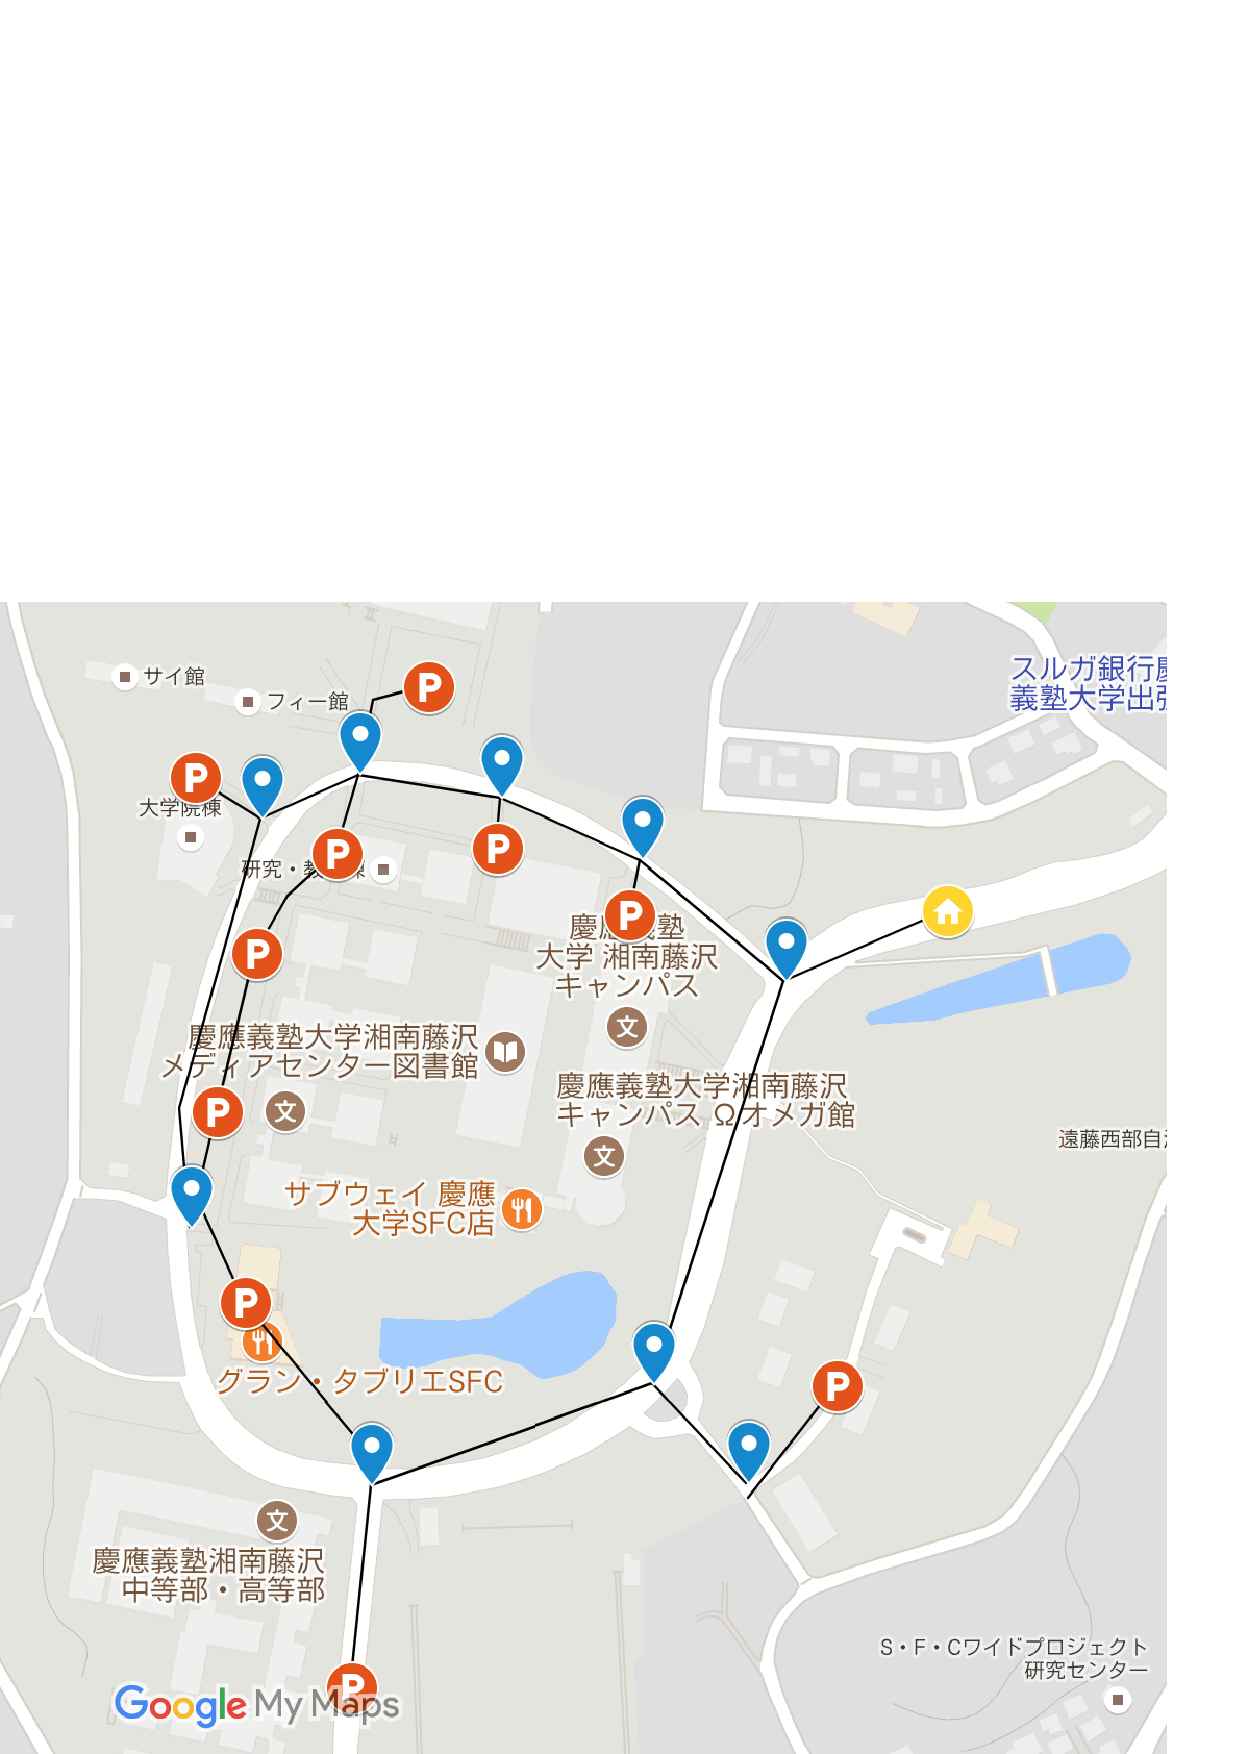
\includegraphics[width=10cm]{fig/google-map.png}
	\caption{googleMaps上にプロットしたSFC内駐車区画のネットワークモデル}
	\label{google-sfc}
\end{figure}


図\ref{sfc-network-model}が本ミュレーター上に再現したSFCのネットワークモデルである.駐車区画を$P$,その他の道路との接続点を$C$としている.車両が駐車場内に進入する箇所を0として,それぞれ19まで識別コードを割り当てる.

\begin{figure}
	\centering
	\includegraphics[width=12cm]{fig/place-sfc.png}
	\caption{ネットワークモデル化したSFC}
	\label{sfc-network-model}
\end{figure}

\subsubsection{各ネットワークノードの特徴}
本評価実験において,各ネットワークノードの駐車枠数や特徴,各駐車場の人気度などは以下の表\ref{sfc-nodes}の通り指定する.
なお,各駐車区画の有する駐車枠数は2018年1月に実施した予備調査で計数したもの,人気度は任意に設定したものである.

\begin{table}[htbp]
	\centering
	\resizebox{\textwidth}{!}{%
		\begin{tabular}{lccclll}
			\hline
			\multicolumn{7}{c}{本評価実験における各ネットワークノードの特徴} \\ \hline
			\multicolumn{1}{c|}{Place ID} & 駐車場 & \multicolumn{1}{l}{駐車枠数} & \multicolumn{1}{l}{人気度} & 座標{[}緯度,経度{]} & 隣接するノードと距離{[}m{]} & 備考                             \\ \hline
			\multicolumn{1}{l|}{0}        & ×        & -                                & -                             & 35.38887,139.4296         & 1:82                                  & スタート地点                 \\
			\multicolumn{1}{l|}{1}        & ×        & -                                & -                             & 35.38857,139.42877        & 0:82,1:82                           &                                    \\
			\multicolumn{1}{l|}{2}        & ×        & -                                & -                             & 35.38908,139.42803        & 1:82,3:26,4:72                    &                                    \\
			\multicolumn{1}{l|}{3}        & ○       & 14                               & 10                            & 35.38885,139.42796        & 2:26                                  & アルファ館横                 \\
			\multicolumn{1}{l|}{4}        & ×        & -                                & -                             & 35.38934,139.4273         & 2:72,5:23,6:67                    &                                    \\
			\multicolumn{1}{l|}{5}        & ○       & 16                               & 5                             & 35.38913,139.42728        & 4:23                                  & シータ館$\cdot$メディア館 \\
			\multicolumn{1}{l|}{6}        & ×        & -                                & -                             & 35.38944,139.42657        & 4:67,7:61,8:39,9:50             &                                    \\
			\multicolumn{1}{l|}{7}        & ○       & 80                               & 5                             & 35.38981,139.42693        & 6:61                                  & 体育館前                       \\
			\multicolumn{1}{l|}{8}        & ○       & 7                                & 20                            & 35.38911,139.42646        & 6:39,11:61                          & ラムダ館横                    \\
			\multicolumn{1}{l|}{9}        & ×        & -                                & -                             & 35.38925,139.42607        & 6:50,10:37,13:197                 &                                    \\
			\multicolumn{1}{l|}{10}       & ○       & 16                               & 15                            & 35.38943,139.42573        & 9:37                                  & タウ館横                       \\
			\multicolumn{1}{l|}{11}       & ○       & 14                               & 25                            & 35.38869.139.42604        & 8:61,12:76                          & イオタ館,オミクロン館  \\
			\multicolumn{1}{l|}{12}       & ○       & 14                               & 10                            & 35.38803,139.42584        & 11:76,13:56                         & カッパ館,イプシロン館  \\
			\multicolumn{1}{l|}{13}       & ×        & -                                & -                             & 35.38754,139.4257         & 9:137,12:56,19:43                 &                                    \\
			\multicolumn{1}{l|}{14}       & ×        & -                                & -                             & 35.38646,139.42663        & 15:95,16:140,19:104               &                                    \\
			\multicolumn{1}{l|}{15}       & ○       & 14                               & 30                            & 35.38561,139.4265         & 14:95                                 & 南門警備室前                 \\
			\multicolumn{1}{l|}{16}       & ×        & -                                & -                             & 35.38688,139.42809        & 1:198,14:140,17:94                &                                    \\
			\multicolumn{1}{l|}{17}       & ×        & -                                & -                             & 35.38646,139.42857        & 16:64,18:67                         &                                    \\
			\multicolumn{1}{l|}{18}       & ○       & 23                               & 15                            & 35.38688,139.42903        & 17:67                                 & テニスコート前              \\
			\multicolumn{1}{l|}{19}       & ○       & 24                               & 5                             & 35.38723,139.42598        & 13:43,14:104                        & 生協棟前                       \\ \hline
		\end{tabular}%
	}
	\caption{SFCの仮想地図内における各区画の属性}
	\label{sfc-nodes}
\end{table}

\subsection{条件設定}
\label{evaluation-test-conditions}
本評価実験の際に設定する条件について記述する.

\begin{itemize}
	\item 1シーケンスの時間 \\
	      本実装では1シーケンスを1秒($t = 1[秒]$)とする.これは利用車両の位置情報送信間隔を1秒と定義することに等しい.
	\item 各仮想車両の目的地の決定\\
	      本シミュレータでは車両が目的の区画で駐車が出来ない場合,他の区画を次の目的地として設定して場内を巡回する.その時,車両は通過した駐車区画に関してその区画の満空状況を確認出来るものとする.また,目的地ではない場合も車両ごとに定められた確率($Car$クラスの$confuse$プロパティ)に依って駐車を試みる.
	\item 仮想車両の駐車時間 \\
	      本評価実験では車両の駐車時間$p_t$は,1時間から3時間($3600[秒] < p_t < 10800[秒]$)までの任意の時間とする.
	\item 各駐車区画の人気度\\
	      各駐車区画の人気度は表\ref{sfc-nodes}で定めたものとする.
	\item 道路$\cdot$交差点の交通量のキャパシティ \\
	      本評価実験では各道路に収容できる交通量を制限しないものとする.仮想車両群は各駐車区画を無制限に通過することが出来る.一方で,区画が保有する駐車枠に空きが無い場合は,駐車を行わず通過するものとする.
	      	
	\item 位置情報ログの生成 \\
	      多様なパターンに対応するため,試行の度にシミュレータを実行し,仮想車両群の位置情報ログデータを生成する.
	\item 試行回数 \\
	      本評価実験では,変数を変える度にシミュレータの実行$\cdot$ネットワークモデルの推定を各説明変数につき100回ずつ行う.
	\item 座標の誤差 \\
	      車両から送信される位置情報に対して第\ref{implementation-send-position}項で述べた誤差付与処理を施す.生成される誤差の分布に関しては図\ref{error-kde}を参照されたい.
	      	
\end{itemize}


\section{評価実験}
\label{evaluation-test-about}
本提案手法の妥当性を検証するために2つの評価実験を行った.本節ではその概要と結果及び考察について述べる.
\subsection{評価実験1:駐車区画の位置推定}
\label{evaluation-test-1}
本項では,第\ref{how-to-park-area}節で述べた駐車区画の位置推定手法を,定量的に評価するための評価実験1について記述する.
\subsubsection{条件と変数}
評価実験1では第\ref{evaluation-test-conditions}節に挙げた条件の他に,以下のような条件を設定する.
\begin{itemize}
	\item 仮想車両のスタート方法\\
		すべての車両を同時にスタート地点から仮想地図内に進入させる.
	\item 最大シーケンス数(収集対象時間) \\
	      評価実験1では最大シーケンス数を設定しない.すべての車両が駐車を完了しSFCから退出するまでの位置情報ログを推定に用いる.
	\item 車両の数\\
	      \ref{evaluation-test-1-var}項に後述するように,評価実験1では仮想地図内に進入する車両の台数を説明変数とする.本実験での車両台数は,実環境下での利用車両の述べ台数とみなすことが出来る.
\end{itemize}
\subsubsection{評価項目}
\label{evaluation-test-1-eval-elements}
評価実験1では,以下の2項目に関して順に推定結果を検証し,推定の成功の可否を検証する.
\begin{enumerate}
	\item 駐車区画の数 \\
	      システムが推定した駐車区画の数と,真値の駐車区画の数が一致するかどうかを検証する.一致した場合次の項目に進む.
	\item 駐車区画の座標 \\
	      システムが推定した各駐車区画の座標群と,真値の座標群との距離が真値の駐車区画間の最短距離より小さい場合,推定が成功したと判断する.
\end{enumerate}

\subsubsection{説明変数と目的変数}
\label{evaluation-test-1-var}
評価実験1では説明変数$x$を仮想地図内に進入する台数とし.推定結果の成功率$y$を目的変数とする.$n$回試行した時の成功率$y$は以下の式のように表される.

なお,本システムの推定機構$f(x)$は推定が成功した場合1を,失敗した場合0を返す.

また,本実験では$x = 50,100,150,200,250,300,350,400,450,500,550,600$,$n=100$とする.

\begin{align}
	y = \frac{\sum_{i=1}^{n} f(x)}{n},x = 車両の台数 \\
	f(x) = 本システムの推定機構                 \\
	n = 総試行回数                                   
\end{align}



\subsubsection{結果}
$x=250$の一度の試行を例に,試行が成功した場合($f(x) = 1$)に,システムが推定した駐車区画の座標とクラスタリング処理を施した駐車時の座標群をプロットした結果を図\ref{evaluation-test-1-success}に示す.青い円は真値の駐車区画座標,線群は真値のネットワークモデルの道路を表すエッジである.

\begin{figure}
	\centering
	\includegraphics[width=14cm]{fig/eval-test-1-success.png}
	\caption{評価実験1が成功したケースにおける推定された駐車区画座標と真値の比較}
	\label{evaluation-test-1-success}
\end{figure}

評価実験1の結果を図\ref{evaluation_test_result_figure}に示す.$x>450$の場合に成功率が$90\%$を超えていることが読み取れる.
\begin{figure}
	\centering
	\includegraphics[width=14cm]{fig/evaluate-result.png}
	\caption{利用車両の台数と推定の成功率の関係性}
	\label{evaluation_test_result_figure}
\end{figure}


\subsubsection{考察}
第\ref{model-case}節より,本実験が対象としたSFCキャンパスの総駐車枠数は222[台]であるため,$90\%$以上の成功率を得るためには,総駐車枠の$200\%$以上の述べ車両台数が必要であることがわかった.1日のうちに駐車区画の多くが満車近くになるSFCの駐車場の場合,データ推定対象となる時間を2日以上に設定することで,十分に信頼できるネットワークモデル推定を行うことが出来ると言える.


\clearpage

\subsection{評価実験2:駐車区画が保有する駐車枠数の推定}
\label{evaluation-test-2}
本項では,第\ref{how-to-park-slot}節で述べた,駐車区画が保有する駐車枠数の推定手法を定量的に評価するための評価実験について記述する.

\subsubsection{条件と変数}
評価実験2では,第\ref{evaluation-test-conditions}節に挙げた条件の他に,以下のような条件を設定する.
\begin{itemize}
	\item 仮想車両のスタート方法\\
	      すべての車両を同時にスタート地点から進入させる.
	\item 最大シーケンス数(収集対象時間) \\
	      評価実験2では最大シーケンス数を設定しない.すべての車両が駐車を完了し,SFCから退出するまでの位置情報ログを本評価実験での推定に用いる.
	\item 車両台数 \\
	      \ref{evaluation-test-1-eval-elements}項で述べたように,評価実験1では,導入する車両台数に最大シーケンス数中の述べ車両台数という意味付けを行った.一方で,評価実験2では場内に存在する最大車両台数と換言する.
	\item 前提となる推定結果 \\
	      駐車枠数の推定を行うためには駐車区画の数$\cdot$座標の2項目が正しく推定されていることが必要である.よって,第\ref{evaluation-test-1-eval-elements}項で定めた基準を満たした場合の推定結果を前提条件とする.
\end{itemize}
\subsubsection{評価項目}
評価実験2では,以下の項目に関して推定結果を検証し,推定の妥当性を検証する.
\begin{enumerate}
	\item 充足率 \\
	      駐車区画$p$に関して,システムが推定した保有枠数$a_p$の真値$G_p$に対する割合を推定充足率$F_p = \frac{a_p}{G_p}$と定義する.$F_p = 1$の時,真値と同じ値を推定したと見なすことが出来る.なお,\ref{how-to-park-slot}項より,$a_p \leq G_p$であるため,$F_p \leq 1 $である.
\end{enumerate}


% 試行回数はn'にしたほうがいい気もする.前提条件があるので
\subsubsection{説明変数と目的変数}
評価実験2では,仮想地図内に進入する車両の台数を説明変数$x$とし,$n$回試行した際の,駐車区画$p$の推定充足率$F_{pn}$の中央値$\tilde{F_{pn}}$を目的変数$y_p$とする.なお,本実験において,$x = 50,100,150,200,250,300,350,400,450,500,550,600$,試行回数$n=100$とする.
\begin{align}
	y_p = \tilde{F}_{pn}                                   \\
	F_{pn} = n回試行した際の推定充足率群      \\
	F_p = \frac{a_p}{G_p}                                  \\
	f_{2}(x,p) = a_p \\
	f_{2}(x,p) = 本推定手法, x = 車両の台数,p = 駐車区画\\
	n = 総試行回数                                    
\end{align}
\subsubsection{結果}
本項では評価実験2の結果について述べる.推定された推定充足率の中央値$\tilde{F_{pn}}$と,車両数$x$との関係を図\ref{slot-result-all-mean-fig}に示す.図\ref{slot-result-boxplots}に各駐車枠ごとの結果を示す.


\begin{figure}[htbp]
	\centering
	\includegraphics[width=14cm]{fig/slot-result-all-mean.png}
	\caption{仮想地図内の最大車両台数と各駐車区画の推定充足率}
	\label{slot-result-all-mean-fig}
\end{figure}

\begin{figure}
	\centering
	\includegraphics[width=16cm]{fig/slot-result-boxplots.png}
	\caption{仮想地図内の最大車両台数と各駐車区画の推定充足率}
	\label{slot-result-boxplots}
\end{figure}

\subsubsection{考察}
図\ref{slot-result-all-mean-fig}より,多くの駐車区画が$x>200$の時,駐車枠数の完全な推定に成功しているケースが多いことが読み取れる.また,人気度の低い2つの区画を除けば,$x>150$の時完全な推測に成功する可能性が高いことがわかる.第\ref{model-case}節より,本実験が対象としたSFCキャンパスの総駐車枠数は222[台]であるため,駐車場内の満車率が$70\%$程度になった場合に,主要な駐車区画の保有する枠数を推定できたと言える.


また,図\ref{slot-result-boxplots}より,区画ID:15やID:11のような特に人気が高い駐車区画に関しては,$x>100$の場合に推測に成功していると言える.人気度が特に高い駐車枠に限れば,満車率が$50\%$程度あれば枠数の把握が可能になることが導かれる.


しかしながら,区画ID:7では,駐車場の総枠数(222[台])以上に車両が場内に進入していても推定充足率が1に満たない.これは,空き枠のある駐車区画があるのにも関わらず,駐車場内を巡回している車両が多く発生していることを意味している.この現象は,各駐車区画の満空状況を各車両が走行中に把握することが出来ない(\ref{evaluation-test-conditions}節を参照)ことが原因であると考えられる.
本評価実験の結果より,人気度が低く枠数が多い駐車区画では,現実的な車両台数では推測できないことが明らかになった.        % 評価

\chapter{結論}
\label{conclusion}
本章では本論文のまとめと今後解決すべき課題を示す.

\section{本研究のまとめ}

本論文では,始めに,路上に敷設した機器を用いる既存の中央管理型駐車場管理システムや,車々間通信による自律分散型管理システムに関する問題点を整理し,その代表として,ネットワークモデルの構築とシステムの管理が運営者の大きな負担であり導入障壁であると指摘した.

次に,既存の研究や手法から,自動車の位置情報を用いる駐車場の最適化手法の有用性を示した.

そこで本研究では,路上に設置する機器や運営主体による管理に依存せずに駐車区画の空き状況を収集$\cdot$可視化出来る環境を創出することを目的として,自動車の位置情報ログデータによって駐車場のネットワークモデルを自律的に推定する手法と,得られたネットワークモデルによって自律的に駐車場の満空状況を管理する新しいアーキテクチャを提案した.

また,駐車場のネットワークモデルを構成する要素を整理し,駐車区画の位置座標と保有する駐車枠数の推定を取り組むべき課題に設定した.本論文では,車両の駐車ログデータとX-Means法を用いたアプローチと,駐車区画の人気度の偏りに注目したアプローチによって自律的に推定する手法を提案した.

加えて,本提案手法の妥当性を検証するために,慶應義塾大学湘南藤沢キャンパスをモデルケースとしたシミュレータを実装し,2つの評価実験を行った.駐車区画の座標に関しては,駐車場の述べ200\%以上のログデータを収集$\cdot$解析することで,十分に信頼できる推定が行えることを示した.また,主要な駐車区画の駐車枠数に関しては,駐車場全体の満車率が70\%程度のログデータを用いることで,高い精度の推定が行えることを示した.

以上の実験の成果として,シミュレータ環境における本提案手法の妥当性が証明された.



\section{将来的な展望}
本論文では妥当性の検証方法として実地図をモデルにしたシミュレータ環境を用いたが,実環境下における有用性は再度検証する余地があると言える.

今後は,実際の車両の走行ログデータや,車載器の低普及環境下での検証を引き続き行い,本提案手法のフィジビリティを明確にしていくことが求められる.

本提案手法の推定精度を更に高めることで,実環境下においても路上常設のセンサーを用いること無く駐車場全体の空き状況の把握$\cdot$可視化$\cdot$最適な区画へのナビゲーションを行うことが可能になり,利用車両の無駄な徘徊の低減や駐車時間の減少を見込める.加えて,都市部や観光地の様な同様の問題が発生しやすい環境下においても,駐車場運営主体の枠を超えた空き状況の統合的な可視化の実現と,渋滞の低減に対する取り組みがが期待される.      % 結論


\chapter*{謝辞}

本論文の執筆にあたり,ご指導いただきました慶應義塾大学政策メディア研究科委員長 村井純博士,環境情報学部教授 楠本博之博士,同学部教授 中村修博士,同学部教授 Rodny D.Van Meter博士,環境情報学部教授 三次仁博士,同学部准教授 植原啓介博士,政策$\cdot$メディア研究科特任准教授 佐藤雅明博士,同研究科特任准教授 鈴木茂哉博士,環境情報学部講師 斉藤賢爾博士,政策$\cdot$メディア研究科特任助教 工藤紀篤博士,同研究科特任助教 空閑洋平博士,同研究科特任講師 松谷健史博士,同元特別招聘教授 下村健一氏,同研究科永山翔太博士に感謝致します.
特に二年次より,研究,外部との共同プロジェクト,学業,進路,私生活の多方面において専らのご指導を賜った佐藤雅明博士,四年次より研究,研究室内ネットワーク管理に関してご指導下さいました植原啓介博士に深謝の意を表します.``インターネット自動車''という興味深い研究テーマを私にご教示戴きました両氏にただただ感謝の限りです.また,遠くハンガリーの地から私の中間発表ポスターにアドバイスを下さいました永山翔太博士,研究のあり方や私生活に関して貴重なアドバイスを下さいました工藤紀篤博士に心よりお礼申し上げます.


また,インターネット自動車研究グループのメンバーとして共に切磋琢磨した,総合政策学部 須田小百合氏,西田亘氏,前田樹氏,環境情報学部 神智尚氏,鈴木雄祐氏,広田和也氏,山田航太郎氏,浅沼沙理氏に深く感謝いたします.特に英語に疎い私を集中特訓してくれた須田小百合氏には感謝してもしきれません.加えて,総合政策学部 深川祐太氏,環境情報学部鈴木雄祐氏,熊谷啓孝氏と取り組んだ外部との研究プロジェクトは私の大きな経験値になりました.諸氏に大変感謝致します.


そして村井研究室での研究,日常生活を共にした優秀な学生の皆様に大変感謝致します.特に,同期の尾崎周也氏,東海林晃氏,河口綾摩氏,桑原誠尚氏,亀井大向氏,神智尚氏,鎧坂文菜氏のような締め切り直前まで生活を共に闘いぬいた「戦友」の存在に日々励まされました.また,先輩として私の研究活動を特にご指導戴きました鈴木恒平氏,加藤桂子氏,阿部涼介氏,小林茉莉子氏,澤井優作氏,大戸浩司氏には特段の感謝の限りです.


最後に,生活,精神両面で多大なる応援をして下さった父 豊田力生氏,母 恭子氏,姉 晏以氏,妹 安莉氏,犬 りんな氏に厚くお礼申し上げます.家族のサポートあってこそ,ここまで生きてこれたといっても過言ではありません.

以上を以って本論文の謝辞とさせていただきます.私を支えて下さった全ての方に重ねて感謝申し上げます.         % 謝辞

\bibliographystyle{unsrt}
\bibliography{b_thesis}

\renewcommand{\thechapter}{\Alph{chapter}}
\setcounter{chapter}{0}
%\appendix


\end{document}
